\documentclass[compress]{beamer}
\usepackage[utf8]{inputenc}
\usepackage{natbib,amsmath,calc,amssymb,graphicx,tabularx,xr,multirow,times,enumitem,array}
%\usepackage[T1]{fontenc}
%\usepackage{default}
\usepackage{hyperref}
\usetheme{Singapore}
% \usecolortheme{beetle}
\definecolor{anthracite}{RGB}{0,0,0}
\definecolor{grey}{RGB}{150,150,150}
\setbeamercolor{background canvas}{bg=anthracite, fg=white}
\setbeamercolor{background}{fg=white, bg=anthracite}
\setbeamercolor{frametitle}{bg=anthracite,fg=white}
\setbeamercolor{title}{fg=white, bg=anthracite}
\setbeamercolor{normal text}{fg=white,bg=anthracite}

% \setbeamercolor{palette primary}{fg=white, bg=anthracite}
% \setbeamercolor{palette secondary}{fg=white, bg=anthracite}
% \setbeamercolor{palette tertiary}{fg=white, bg=anthracite}
% \setbeamercolor{palette quaternary}{fg=white, bg=anthracite}
\setbeamercolor{local structure}{fg=white, bg=anthracite}
\setbeamercolor{structure}{fg=white, bg=grey}
\setbeamercolor{section in head/foot}{fg=white, bg=anthracite}

\usepackage[T1]{fontenc}


%add the little bullets for the slides
\useoutertheme{miniframes}
\usepackage{etoolbox}
% \usepackage{enumitem}
\usepackage{multimedia}
\makeatletter

%%%%
%%%% THIS MAKES SOME NAVIGATION CYRCLES DISAPPEAR BY USING THE COMMANDS \miniframesoff or \miniframeson : useful for skipping title slide or when there are too many slides
%%%%
\useoutertheme[subsection=false]{miniframes}
\let\beamer@writeslidentry@miniframeson=\beamer@writeslidentry
\def\beamer@writeslidentry@miniframesoff{%
  \expandafter\beamer@ifempty\expandafter{\beamer@framestartpage}{}% does not happen normally
  {%else
    % removed \addtocontents commands
    \clearpage\beamer@notesactions%
  }
}
\newcommand*{\miniframeson}{\let\beamer@writeslidentry=\beamer@writeslidentry@miniframeson}
\newcommand*{\miniframesoff}{\let\beamer@writeslidentry=\beamer@writeslidentry@miniframesoff}
%%%
%%%

%% essential for showing the bullets!!
\usepackage{remreset}
\@removefromreset{subsection}{section}
\setcounter{subsection}{1}
%%

\setbeamertemplate{navigation symbols}{}

\makeatother

% title page info
\title[CPM]{\large \textbf{Modeling development with Cellular Potts Model}} %axis extension and segmentation
% \subtitle{Evo-devo models of sequential segmentation}
\date{}
\titlegraphic{\vspace*{-12mm}\includegraphics[width=0.5\textwidth]{figures/titlepage.png}}
\author{Renske Vroomans}
%\author{Supervisors: Kirsten ten Tusscher \& Paulien Hogeweg} 
\begin{document}
 
 
%slide 1
\miniframesoff
 
\begin{frame}[plain]
\titlepage
\end{frame}
%say a bit about myself: worked with CPM during my Master's and beginning of PhD, went on to evo-devo models of animal segmentation
\miniframeson

\section{About me}

\begin{frame}
\frametitle{Master's and PhD in Utrecht}

\begin{itemize}
 \item T cell migration
 \item Plant hormones in fruit development
 \item Evo-devo of animal segmentation
 \item Tcell receptor sequences in database
\end{itemize}

\end{frame}


\begin{frame}
\frametitle{Currently: EmbryoMaker}
 \begin{center}
     \includegraphics[width=0.5\textwidth]{figures/embryomaker_init.png}
     \includegraphics[width=0.5\textwidth]{figures/embryomaker_exp.png}\\
     \tiny Marin-Riera \textit{et al.,} 2015
     \end{center}
\end{frame}

\begin{frame}
\frametitle{Epithelial morphologies}
 \begin{center}
     \includegraphics[width=0.5\textwidth]{figures/embryomaker_phen.png}
     \end{center}
\end{frame}


\begin{frame}
 \frametitle{Acknowledgments}
 
 My CPM teachers and mentors:\\
 Paulien Hogeweg\\
 Joost Beltman\\
 Stan Mar\'ee\\
 Ramiro Magno\\
 Roeland Merks\\
 \vspace*{1cm}
 My guinea pigs:\\
 Marie M\"uller\\
 Vilma Väänänen\\
 Aida Kaffash Hoshiar\\
 
\end{frame}

\section{Prelude}
% slide 2: EXTEND!!
\begin{frame}
  \frametitle{Why do we make models}
  \begin{itemize}
   \item to inform the next experiment
   \item to test difficult hypotheses
   \item to identify gaps in our knowledge %when things go wrong or as a way of thinking clearly; all models are wrong, some are useful
   \item to understand mechanism and process %more data is not necessarily more insight
   \item to be surprised
  \end{itemize}
 lower-level properties <--> higher-level phenomena\\
 
 \begin{center}
     \includegraphics[width=0.5\textwidth]{figures/fokke_sukke.JPG}\\
     \tiny (C) John Reid and Bastiaan Geleijnse
     \end{center}
 
\end{frame}

\begin{frame}
\frametitle{What should a model of cells capture?} 
 
 short answer: that depends on the question %Paul discussed this yesterday
 \\~\\
 CPM is suitable for mesoscale cell modeling:\\
 between cells as points and cells as complex machines\\
 
\end{frame}

\begin{frame}
\frametitle{What should a mesoscale model of cells capture?} 

 \begin{columns}
    \begin{column}{0.49\textwidth}
    \vspace*{-1cm}
    
    \begin{center}
     \includegraphics[width=0.8\textwidth]{figures/cellshape.png}\\
     \end{center}
     \small Cells have a size and shape\\
     \small Cells can be more or less stiff\\
     \small They experience 'spontaneous' membrane fluctuations\\
     \small They can be more or less motile\\
    \end{column}
    \begin{column}{0.49\textwidth}
    \small Cells can interact and adhere  \\
    \vspace*{-0.25cm}
    \begin{center}
  \includegraphics[width=0.6\textwidth]{figures/interactions.png}\\
  \tiny taken from http://pathmicro.med.sc.edu/lecture/hiv7.htm \\
  \vspace*{-0.2cm}
     \end{center}
     \small divide or cleave, grow and die\\
%       \vspace*{-0.3cm}
      \small They have a gene expression state\\
      \vspace*{-0.35cm}
     \begin{center}
  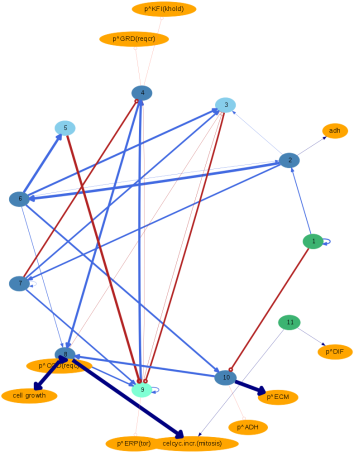
\includegraphics[width=0.4\textwidth]{figures/grn.pdf}\\
     \end{center}
     
    \end{column}
   \end{columns}

%  Cells have a size, a shape, a chemical composition, a gene expression state, internal compartments
%  Determine physical properties like stiffness, stickiness, motility
%  Are viscous
% Resist shape change, but can still be compressed
% Rapidly redistribute pressure

\end{frame}
 
 \section{Basic CPM}
 \begin{frame}
 \frametitle{The CPM as a mesoscale cell model}
 
 \begin{center}
  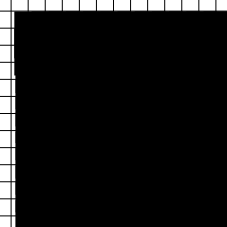
\includegraphics[width=0.6\textwidth]{figures/cpm_layout.pdf}\\
     \end{center}
 
 %Size and shape are r - intracellular compartments often less so.
Each cell is a distinct unit --> cell id $\sigma$\\ %shape and volume due to multiple points
Cells can have a type ($\tau$)%, determining global cell properties like size and adhesion.

 \end{frame}

\begin{frame} 
\frametitle{The heart of CPM: the Hamiltonian}
% The principle that drives the dynamics of CPM is that of energy minimisation.
% A cell is subject to forces from the environment (other cells) and internal forces (pressure, membrane)
% deformation of cells due to fluctuations and the resolution of global and local forces.
% Describe this implicitly with the Hamiltonian.
Dynamics due to energy minimisation and random fluctuations\\
The Hamiltonian, $H$, describes the total energy of the system\\ 
Monte Carlo step: consider for each pixel whether a neighbour will copy into it: probability determined by change in $H$\\

\begin{equation}
P_{1->2}=\begin{cases}
    1, & \text{if $\Delta H \leq 0$}.\\
    e^{\frac{-\Delta H}{T}}, & \text{if $\Delta H>0$}.
  \end{cases}
\end{equation}

% \begin{center}

\begin{columns}
    \begin{column}{0.49\textwidth}
    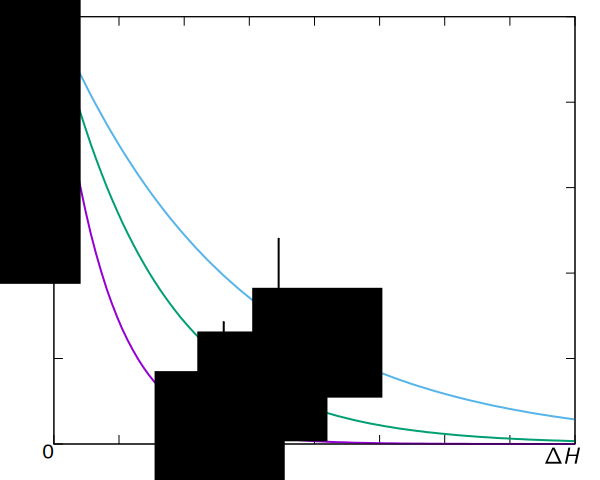
\includegraphics[width=0.9\textwidth]{figures/copyprob.pdf}
     \end{column}
    \begin{column}{0.49\textwidth}
   \movie[poster,loop]{ \includegraphics[width=0.8\textwidth]{figures/copy_event.png}}{onecell.mp4}
    \end{column}
   \end{columns}
\end{frame} 

\begin{frame}
 \frametitle{The energies in basic CPM}
 
 \begin{center}
  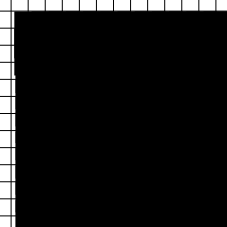
\includegraphics[width=0.5\textwidth]{figures/cpm_layout.pdf}\\
     \end{center}
 
intracellular pressure: deviations from resting volume\\
energy from the interface between cells: adhesion-driven membrane tension
 \end{frame}
% \end{center}

\begin{frame}
\frametitle{Capturing cell volume preservation in CPM}  
% A term in the hamiltonian ensures that, while cell volume may fluctuate (cells are compressible), they want to 
% without active input, cells prefer to stay roughly the same size.
\[H = \lambda ( a - A)^2\]

For all cells:
$$ H = \sum_\sigma \lambda ( a_\sigma - A_{\tau(\sigma)}  )^2 $$
  
  

\end{frame}

 \begin{frame}
\frametitle{Capturing adhesive cell interactions in CPM}   
\begin{center}
  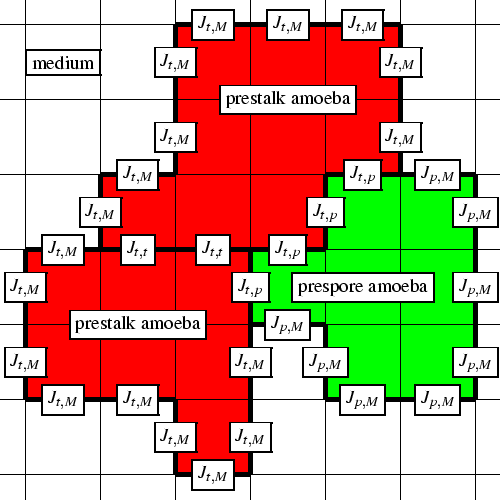
\includegraphics[width=0.5\textwidth]{figures/explanation.pdf}
\end{center}
Whether cells adhere depends on the interaction energy $J$, defined per unit contact length.\\
J values are typically defined between cell types\\
% The higher the energy, the less likely they are to stay in contact.\\
% It is a balance of energies between different cell types --> 
touching medium also has an associated energy
 
\end{frame}

 \begin{frame}
\frametitle{Capturing adhesive cell interactions in CPM}   

\begin{multline}
 H = \sum_\sigma \lambda ( a_\sigma - A_{\tau(\sigma)}  )^2\\
+ \sum_{all\,\sigma,\sigma'} \frac{J_{\sigma,\sigma'}}{2}\\
+\sum_{all\,\sigma,medium} J_{\sigma,medium}
\end{multline}
\end{frame}

\begin{frame}
\frametitle{To stick or not to stick}   


\begin{center}
%   \includegraphics[width=0.3\textwidth]{figures/copy_event.png}\\
$J_{cell,med}<J_{cell, cell}$ ~~~~~ $J_{cell,med}>J_{cell,cell}$
\movie[width=5cm, height=5cm, poster, loop]{\includegraphics[width=0.45\textwidth]{figures/brokenheart.png}}{slide1.2.mp4}
\movie[width=5cm, height=5cm, poster, loop]{\includegraphics[width=0.45\textwidth]{figures/heart.png}}{slide1.1.mp4}
\end{center}

Energy minimisation leads to ball shape of entire tissue
\end{frame}

\begin{frame}
\frametitle{Differential adhesion hypothesis}   
\begin{center}
  \includegraphics[width=0.5\textwidth]{figures/cnidarians.jpg}
\end{center}
Hypothesis: tissues behave like immiscible fluids\\
% mixed aggregates would sort out 
How to test this with CPM?\\

\end{frame}


\begin{frame}
\frametitle{Commands}   
\begin{itemize}
 \item \texttt{sudo dpkg-reconfigure keyboard-configuration}
 \item copy directory from USB stick to your home directory
 \item \texttt{cd practicum}
 \item \texttt{evince exercises.pdf}
\end{itemize}
Before starting the exercises:
\begin{itemize}
 \item \texttt{cd pkgs}
 \item \texttt{sudo dpkg -i *.deb} (this may take some time)
 \item \texttt{cd ../cpmcode  }
 \item \texttt{make}
\end{itemize}
to run code:\\
\texttt{./bin/CPM -d DIRNAME -s SEED parfile.cfg}
\end{frame}


\end{document}
